
\documentclass{kais}
%
\usepackage{wrapfig,epsf}
\usepackage[dcucite]{harvard}

\usepackage{mathtools}
\usepackage{color}
\usepackage{graphicx}
\usepackage{courier}
\usepackage{listings}

\lstset{basicstyle=\small\ttfamily} 

\newtheorem{defi}{Definition}[section]
\newtheorem{property}{Property}[section]
\newtheorem{algorithm}{Algorithm}[section]

\newcommand\changenum{%
  \renewcommand\labelenumi{\theenumi}%
  \renewcommand{\theenumi}{(\arabic{enumi})}%
}

\newcommand\changepnum{%
  \renewcommand\labelenumi{\theenumi}%
  \renewcommand{\theenumi}{($P_\arabic{enumi}$)}%
}

\bibliographystyle{agsm}
\citationmode{abbr}

% For commenting
%\newcommand{\comment}[1]{{\small \color{red} {#1}} \normalcolor}
% Use this line for leaving out comments
\newcommand{\comment}[1]{}

% Todo
%\newcommand{\todo}[1]{{\small \bf \color{blue} {#1}} \normalcolor}
% Use this line to leave out
\newcommand{\todo}[1]{}

% Notation commands (change all by changing here)
% Defina a capital Rho
\newcommand{\Rho}{\mathrm{P}}
% Concept relation
\newcommand{\rn}[1]{\rho_{#1}}
% Concept L1 norm
\newcommand{\rns}[1]{|\rn{#1}|_1}
% Concept relation threshold
\newcommand{\mrn}[1]{\tau_{#1}}
% Discarded concept relation sum
\newcommand{\drns}[1]{|\check{\rho}_{#1}|_1}
% Kept concept relation sum
\newcommand{\krns}[1]{|\hat{\rho}_{#1}|_1}
% Concept relation vector
\newcommand{\rv}{\Rho}

% Concept similarity
\newcommand{\sy}[1]{\sigma_{#1}}
% Approximate concept similarity
\newcommand{\asy}[1]{\tilde{\sigma}_{#1}}
% L1 norm of difference
\newcommand{\nm}[1]{L_1(#1)}
\newcommand{\dnm}[2]{|\rn{#1}-\rn{#2}|_1}
% Approximate L_1 norm
\newcommand{\anm}[1]{\tilde{L}_1(#1)}

\received{xxx}
\revised{xxx}
\accepted{xxx}

\pubyear{xxx}
\pagerange{\pageref{firstpage}--\pageref{lastpage}}
\volume{xxx}

\begin{document}
\label{firstpage}

%\title{Knowing an Object by the Company It Keeps: A Domain-Agnostic Scheme for Similarity Discovery}
\title{Knowing an Object by the Company It Keeps: Discovering Similarities and Concepts from 
Contexts\footnote{This paper is an extended version of \cite{Gornerup2015}, to be presented at ICDM 2015.}}
\shorttitle{Knowing an Object by the Company It Keeps}

\author[O. G\"{o}rnerup et al]{Olof G\"{o}rnerup$^1$, Daniel Gillblad$^1$ and Theodore Vasiloudis$^1$\\ 
$^1$Swedish Institute of Computer Science (SICS), Kista, Sweden}

\maketitle

\begin{abstract}
Appropriately defining and then efficiently calculating similarities from large data sets are often essential
in data mining, both for gaining understanding of data and generating processes, and for building tractable representations.
Here we rely on the premise that, given a set of objects and their correlations, each object is characterized
by its context, i.e.\ its correlations to the other objects. The similarity between two objects can therefore be 
expressed in terms of the similarity between their contexts. In this way, similarity pertains to the basic 
and general notion that objects are similar if they are exchangeable in the data. Resting on these principles, we propose a 
data-driven and highly scalable approach for discovering similarities from large data sets by representing objects 
and their relations as a correlation graph that is
transformed to a similarity graph. Together these graphs can express rich structural properties
among objects. Specifically, we show that concepts -- generalizations and abstractions of
data -- are constituted by groups of similar objects that can be identified
by clustering the objects in the similarity graph.
These principles and methods are applicable in a wide range of fields, and will here be demonstrated 
in three domains: computational linguistics, music and molecular biology, where the numbers of objects and correlations
range from small to very large.
\end{abstract}

\begin{keywords}
Similarity discovery; Concept discovery; Distributional semantics
\end{keywords}

\section{Introduction}
\label{sec:introduction}

As stated by \citeasnoun{Firth57} and further popularized in the computational linguistics community by \citeasnoun{Church90}, 
``You shall know a word by the company it keeps''. Based on this principle, which can be 
traced further back to analytic philosophy, there have been substantial efforts to infer semantic and syntactic meaning
 from words through their effective usage in text \cite{Harispe2015}. Although the same principle has been applied in 
 different and seemingly distinct domains, such as bibliometrics  \cite{Kessler1963} and bioinformatics 
 \cite{ravasz2002hierarchical}, generalizing the notion of characterizing objects through 
their contexts into a broader fundamental principle for similarity discovery is so far largely unexplored.

Extending Firth's line of thought we argue that the effective semantics of any object, with respect to observed data, are characterized 
by the context in which it occurs, or in other words, by how it is related (or correlated) to all other objects. The \emph{similarity} 
between two objects may therefore be formulated in terms of their contexts, or how similar their relations to all other
objects are.
A benefit of this is that we can omit the specific functionality or underlying workings of objects, but
only observe and consider their context patterns. This is highly attractive from a data-driven machine learning
perspective since it requires very few assumptions about the objects.

With this as a starting point, we propose a graph-based method for discovering similarities from large data
sets. An \emph{object} is intentionally left vague since it can be many different things, such as
music tracks in a playlist, people in a social network, tokens in a text or states in a stochastic process. We narrow down the scope
slightly by only considering objects that exhibit pairwise relations, e.g.\ in terms of spatial, temporal or social
correlations, which allows us to represent a collection of objects and their inter-dependencies as a graph. Our
approach, which we call \emph{Contextual Correlation Mining} (CCM), involves two main steps: First, we create a \emph{correlation graph} 
that describes the pairwise correlations between all objects. A correlation may here be any relationship measure such as the frequency 
of co-occurrence, a transition probability in a stochastic process, a correlation measure such as mutual information or a weighted edge in a graph. 
Second, we transform the correlation graph to a \emph{similarity graph} by comparing the set of correlations of each object
to the sets of correlations of all other objects -- the more similar sets of correlations, the higher the weighted edge in the
similarity graph.

The correlation graph is either given at the outset, as a Markov model or co-occurrence network for example, or built from data.
Since there already exists a multitude of approaches for achieving this, see e.g. \cite{Albert2002}, we will here focus on the second 
step, which we also view as the main technical contribution of this paper. Transforming a correlation graph to a similarity graph 
is conceptually straightforward, but as an ``all-to-all" similarity
problem, it is highly challenging in practice. However, since we are considering
pairwise correlations, we can utilize that similar objects always occur in proximity in the correlation graph (at most one neighbour apart to 
be specific), which means that it is sufficient to compare objects locally in the graph. This not only drastically reduces the number 
of necessary comparisons,
but also facilitates parallelization. Moreover, given that the correlation graph is sparse\footnote{That is, most objects are 
either completely unrelated or at most negligibly correlated. Two randomly selected persons in a large social network, for 
instance, most likely do not know each other.} -- which is the case e.g.\ for gene co-expression \cite{Jordan2004}, semantic
 \cite{Steyvers2005}, word co-occurrence \cite{Cancho2001} and social networks \cite{mislove2007social}, as well as for 
 many other graphs of interest \cite{Albert2002} -- we can also prune the correlation graph substantially 
prior to transforming it to a similarity graph while keeping the approximation error low and controllable.

In comparison, related methods are either limited to specific domains 
or do not scale well with growing number of objects, while the approach presented here is both highly scalable and agnostic
with respect to objects and correlation measures. These are merely seen as vertices and edges in a graph, and CCM
is therefore applicable in a broad range of domains as well as in mixed-data scenarios where several different correlation measures
may be considered. In this way, we propose a powerful and efficient scheme that distills the essence in many related, and seemingly 
distinct, methods by using the core principle that objects can be characterized by the contexts in which they occur.

Furthermore, since CCM does not require any intermediate representations of objects and their correlations, such as sparse vectors
 or neural networks, it is also interpretable and transparent. This enables us to calculate well-understood notions
of similarity and error among other things. Representing objects, correlations and similarities as graphs will also allow us
 to capture rich higher-scale structures among objects -- e.g.\ without being constrained by geometric properties such as the triangle 
inequality -- including ambiguity, hierarchies and ontologies, both in terms of correlations and similarities.
Rather than representing data in terms of its raw constituents, a central task then is often to discover appropriate levels of abstraction 
of objects, both for gaining insights about data and by computational necessity. As an illustrative example, it may 
for instance not be suitable to analyze a large text corpus in terms of its individual characters, when the data can be described in 
terms of words or on more abstract levels still. We will here demonstrate that CCM can be used for this purpose. Specifically, we will show 
that \emph{concepts} -- abstract generalizations of objects -- are constituted by groups of inter-similar objects that play 
analogous roles in data, and that we can discover these by clustering the objects in the similarity graph. 

\subsection{Outline}
The remainder of the paper is outlined as follows: Next we will put the paper in context by giving an overview of the related
state-of-the-art. A background with preliminaries is presented in Sec.\ \ref{sec:background}, followed by a description of the
proposed method in Sec.\ \ref{sec:methods}, including theoretical investigations on error bounds and scalability. 
In Sec.\ \ref{sec:experiments} we demonstrate the versatility of the method by
applying it in three distinct domains -- computational linguistics, music and molecular biology -- and present experimental evaluations
of the method's accuracy and scalability. The paper is concluded in Sec.\ \ref{sec:conclusions} with a summary of our findings 
and a discussion on possible future directions.

\section{Related work}
\label{sec:related work}

The principle of relating objects with respect to contextual information is employed in several different areas, including ontology
learning, computational linguistics, bioinformatics and bibliometrics. The method that is closest in spirit to
ours is SimRank \cite{Jeh2002simrank}, which is a general approach for obtaining similarities between vertices in a graph.
SimRank is an iterative method that uses the graph structure to derive similarities between objects by relating ``objects that are
related to similar objects'' \cite{Jeh2002simrank}. The main drawback with their approach, however, is that it is not scalable due to
a cubic time complexity with the number of vertices in the graph. This has partly been remedied in improved versions of the algorithm,
such as the one by \citeasnoun{Yu2012simrankOpt}, but these are still too computationally demanding in order to be applicable on
very large graphs. In comparison, we can comfortably run our algorithm on substantial graphs, doing only a single
pass over the data.
\citeasnoun{leicht2006vertex} propose a similarity calculation method which deals with another
limitation of SimRank, namely that similarities are only calculated for nodes connected by paths of
even length. The authors propose an alternative iterative method, but it suffers from much of the same scalability
problems as with SimRank.
\citeasnoun{ravasz2002hierarchical} propose an approach for finding similar vertices using so called
topological overlap measures, which they apply on metabolic networks. \citeasnoun{Zhang2005tom}
generalized this approach for use on weighted gene co-expression networks. As in our case, these methods relate vertices by assigning
higher similarity scores between vertices that share many neighbors, but since their approaches are primarily tailored for bioinformatics tasks,
they lack the generality of SimRank and the method presented here.
  
In computational linguistics, distributional analysis -- where linguistic items are characterized by
their relative distributional properties in the data -- has become a fundamental approach \cite{Harris-1970}. We use
similar assumptions as a starting point, and when applied to text, the approach can be seen as transforming a graph
over syntagmatic similarities to one describing paradigmatic similarities \cite{Sahlgren-2006}, in which
concepts are discovered through clustering. A large number of methods to find semantic similarities have been
developed -- see \cite{Harispe2015} for a recent review -- from the seminal work by \citeasnoun{Church90}, and \citeasnoun{Brown1992}, to more recent approaches, e.g.\ based on vector representations, such as GloVe 
\cite{Pennington2014}, and neural networks, such as word2vec \cite{Mikolov-2013}. 
Several of these methods could be used to produce the equivalent of the similarity graph on which we perform
clustering to find concepts. These methods, however, are limited to natural language processing while our approach 
is domain-agnostic. Another important difference is that our method builds similarity graphs without 
using any dimensionality reduction or intermediate representations, such as high-dimensional vectors 
or difficult-to-interpret neural networks. The advantage of using a direct graph representation is that it allows us to
understand and reason about higher-scale structures among objects and concepts, such as hierarchical organization, in a straightforward 
manner using established graph and network methods. Although graph representations are used in natural language processing to relate 
similar words and documents \cite{Mihalcea2011}, these approaches have several limitations in comparison to our 
approach, e.g.\ by expecting existing similarity graphs as input, using ad hoc word relations (such as linking words separated 
by \emph{and} or \emph{or}), requiring part-of-speech tagged data, or by using human curated datasets, such as WordNet \cite{miller1995wordnet}.

Another related area is ontology learning \cite{Wong2012ontology}, which aims to infer taxonomies 
from corpora and other data sources. While one can draw parallels between our work and this field, the latter is often limited 
by exclusively considering a specific type of basic building blocks, such as nouns, where these are related in 
 hierarchies with respect to specific relations, such as \emph{is a} and \emph{part of}. Similarly, context-based similarity
  discovery can also be viewed as a generalization of methods in bibliometrics, where citation patterns among a set of 
  documents, such as scientific papers, are studied. Using so called bibliographic coupling to relate papers  \cite{Kessler1963} 
  -- i.e.\ the similarity between two papers is based on the number of  citations they share -- is a special case of our approach 
  for relating two objects in the correlation graph. Another resemblance is that  these and similar measures are used to cluster 
  scientific papers \cite{Small1973} as well as web pages \cite{Larson96}. The method presented here could be employed in 
  the very same way -- where binary correlations are given by citations -- to efficiently relate a large number of documents.

\section{Background}
\label{sec:background}

\subsection{Preliminaries}
\label{sec:preliminaries}

We begin by specifying the terminology used in this paper. Due to the transdisciplinary character of the method, we
 choose to use general rather than domain-specific terms.

Let $C = \{i\}_{i=1}^n$ be a set of \emph{objects}, where each object has a correlation, $\rn{i,j}$, to
each other object. This relation can be expressed in terms of real values, probabilities, booleans or something
else that, for instance, represent a correlation measure, binary or weighted neighbourhood relation in a graph,
co-occurrence probabilities in a corpus, or transition probabilities in a Markov chain. An object can for example be a 
word in text, and the correlations between words can be their co-occurrence probabilities. In another example, objects 
constitute people, and the correlation between two persons is their strength of acquaintance.

The \emph{context} of an object $i$ is considered to be its vector of relations to every other object, $\rn{i} =
(\rn{i,j})_{j=1}^n$. In our word example, the context of a word is therefore its correlations to all other words. Analogously, 
in the people example, the context of a person is all that person's acquaintances.

Under the assumption that an object is characterized by its context, we can formulate the
similarity between two objects $i$ and $j$, denoted $\sy{i,j}$, in terms of a similarity measure between their
respective contexts.
Here we define $\sy{i,j}$ to be 1 subtracted by the relative $L_1$-norm of the difference between $\rn{i}$ and $\rn{j}$:
\begin{equation}\label{eq:sim}
\sy{i,j} = 1 - \frac{\dnm{i}{j}}{\rns{i} + \rns{j}},
\end{equation}
where
\begin{equation}\label{eq:totrel}
\rns{i} = \sum_{k \in C} | \rn{i,k}|
\end{equation}
and
\begin{equation}\label{}
\dnm{i}{j} =  \sum_{k \in C} | \rn{i,k} - \rn{j,k} |,
\end{equation}
denoted $\nm{i,j}$ for short.
That is, we normalize the absolute $L_1$-norm of the difference between $i$ and $j$:s context vectors with the maximum
possible norm of the difference, as given by $\rns{i} + \rns{j}$, and then subtract the result from one in order to
transform it to a similarity measure bounded by 0 and 1, $\sy{i,j} \in [0, 1]$.

Since objects are discrete and have pairwise relations, we can represent $C$ and $\rn{i,j}$ as a directed graph,
$\mathcal{R} = (C, R)$, where vertices constitute objects, and where edges $r_{i,j} \in R$ have weights $\rn{i,j}$. We
term this the \emph{correlation graph} of $C$ with respect to $\rn{i,j}$. In principle this is a complete graph since
every vertex has a relation to every other vertex (including itself) through $\rn{i,j}$. However, we define the graph
such that there is only an edge between two vertices $i$ and $j$ if their corresponding objects have a degree of
similarity, i.e.\ when $\dnm{i}{j} < \rns{i} + \rns{j}$ and $i \neq j$. In our people example, the correlation network 
is simply a acquaintance network.

Analogously, the \emph{similarity graph} of $C$ with regard to $\rn{i,j}$, denoted $\mathcal{S} = (C, S)$, is defined
to be an undirected graph where weights of edges $s_{i,j} \in S$ instead are given by $\sy{i,j}$.

By \emph{concept} we mean a group of objects that are approximately similar -- forming a cluster in 
the similarity graph -- and therefore approximately interchangeable in their respective contexts. In the word example 
this may correspond to a group of semantically and/or syntactically similar words (e.g.\ termed \emph{semantic community} 
or \emph{topic} in the natural language processing community), whereas in the people example, a concept is a group of 
people that have similar circles of acquaintances, such as a group of colleagues.

\subsection{Example}

\begin{figure}
\centerline{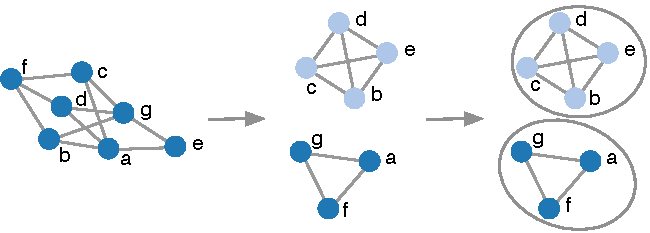
\includegraphics[width=0.65\columnwidth]{figures/examplegraphs.pdf}}
\caption{A correlation graph is transformed to a similarity graph in which clustering is performed.}
\label{fig:examplegraphs}
\end{figure}

As a simple stylized example, consider the set of objects $C = \{a,b,c,d,e,f,g\}$ with the symmetric, binary correlation 
graph shown to the left in Fig.\ \ref{fig:examplegraphs}. Transforming this correlation graph to the similarity graph shown in 
the same figure using Eq.\ \ref{eq:sim}, the pairwise similarities become positive when two objects have overlapping contexts. 
Each of the two clusters in the similarity graph is then identified as a concept.

Note that in the case of the binary relationship graph, the $L_1$-norm between two objects, $i$ and $j$, is given by the 
number of neighbours that they do not share:
\begin{equation}
\dnm{i}{j} = |n_i \cup n_j| - |n_i \cap n_j| = |n_i| + |n_j| - 2 |n_i \cap n_j|,
\label{eq:binarynorm}
\end{equation}
where $n_i$ and $n_j$ are the neighbourhoods of $i$ and $j$. Since the maximum possible norm of the difference is $|n_i| + |n_j|$, 
the similarity between $i$ and $j$ becomes
\begin{equation}
\sy{i,j} = 1 - \frac{|n_i| + |n_j| - 2 |n_i \cap n_j|}{|n_i| + |n_j|} = \frac{2 |n_i \cap n_j|}{|n_i| + |n_j|},
\label{eq:binaryrelnorm}
\end{equation}
which is known as the S{\o}rensen-Dice coefficient \cite{Dice45,Sorensen48}, that, in turn, is analogous to the commonly 
used Jaccard coefficient \cite{Jaccard1912} through a monotonic transformation.

\section{Methods}
\label{sec:methods}

\subsection{Similarity calculations}
\label{sec:similaritycalculations}

In order to efficiently and scalably transform a correlation graph into a similarity graph, we utilize two observations
concerning the correlation graph with regard to locality and sparseness. 
Firstly, according to our definition of similarity, an object only has a degree of similarity to its second-order
neighbours (its neighbours' neighbours) in the
correlation graph $\mathcal{R}$. Let $n_i$ and $n_j$ be the neighbouring vertices of $i$ and $j$ respectively, and $\rn{i,
k} = 0$ if $k \not\in n_i$. Then
\begin{eqnarray}
\nm{i,j}  & = &
\sum_{k \in n_i}  |\rn{i, k}| -  \sum_{\mathclap{k \in n_i \cap n_j}}  |\rn{i, k}|
+  \sum_{k \in n_j}  |\rn{j, k}| -  \sum_{\mathclap{k \in n_i \cap n_j}}  |\rn{j, k}|
+  \sum_{\mathclap{k \in n_i \cap n_j}} |\rn{i, k} - \rn{j, k}| \notag\\
& = & \rns{i} + \rns{j} + \Lambda_{i,j}, 
\label{eq:l1terms}
\end{eqnarray}
where
\begin{equation}
\Lambda_{i,j} = \sum_{\mathclap{k \in n_i \cap n_j}} (|\rn{i, k} - \rn{j, k}| - |\rn{i, k}| - |\rn{j, k}|)
\label{eq:l1common}
\end{equation}
When calculating Eq.\ \ref{eq:sim} it is therefore sufficient to compare differences between weights $\rn{i, k}$ and
$\rn{j, k}$ of edges from $i$ and $j$ to neighbours $k$ that $i$ and $j$ have in common, given that we have the weight
sums of outgoing edges of $i$ and $j$.
In practice, we generate a similarity graph by first summing weights of outgoing edges per vertex, and then building an
intermediate undirected two-hop multigraph of $\mathcal{S}$, where an edge $(i, j)$ that corresponds to a hop through
$k$ in $\mathcal{S}$ has weight $|\rn{i, k} - \rn{j, k}| - |\rn{i, k}| - |\rn{j, k}|$. The $L_1$-norm between $i$ and
$j$ is then calculated by summing the weights of all edges between $i$ and $j$ in the multigraph according to Eq.\
\ref{eq:l1common}, and adding this to the edge weight sums of $i$ and $j$.

Just as our approach is applicable for different correlation measures, it is not strictly limited to the $L_1$-norm. Using 
other distance measures is also possible, given that these can be decomposed in a way akin to Eq.~\ref{eq:l1terms}. 

\subsubsection{Approximations}
\label{sec:approximations}
Even though we only need to consider shared neighbours when calculating the similarities between objects, these
calculations still scale unfavorably as the sum of the square of in-degrees per vertex, since we consider all pairs of
incoming edges of vertex $k$ when generating two-hop edges. We therefore need to approximate the similarity measure by
reducing in-degrees. To be able to determine whether a certain object distance with respect to a distance measure $D$ is
relevant or not, typically we would like to ensure that the error $E_{D}(i,j)$ in any specific distance approximation
is less than a fixed level $\theta_D$,
\begin{equation}
E_{D}(i,j) \leq \theta_D
\end{equation}
and more specifically for the $L_1$-norm approximated by $\tilde{L}_1$,
\begin{equation}
E_1(i,j) = | \nm{i,j}  - \anm{i,j}  | \leq \theta_1.
\end{equation}
If we would like to remove terms by approximating by zero while keeping the total approximation error $E_1(i,j)$ 
as small as possible, we should remove the smallest absolute correlation terms $|\rn{i,k}|$ in Eq.\ \ref{eq:l1terms}. Put differently,
we discard the edges with the smallest weights in the correlation graph.
Let $\mrn{i}$ be a threshold value below which absolute correlations of object $i$ are approximated by zero, and $\drns{i}$ the 
norm of discarded correlations:
\begin{equation} \label{}
\drns{i} = \sum_{ |\rn{i,k}| < \mrn{i}} |\rn{i,k}|.
\end{equation}
The upper bound of the error is then given by
\begin{equation} \label{eq:errbound}
E_1(i,j) \leq \drns{i} + \drns{j},
\end{equation}
where $E_1(i,j)=\drns{i} + \drns{j}$ when the edges of discarded relations of $i$ and $j$ do not share any destination
vertex $k$. When calculating the object similarity based on the $L_1$-norm, we can therefore reduce the number of
terms we need to compare by removing low correlation values with predictable errors. Lowering the number of terms in
Eq.\ \ref{eq:l1common} while guaranteeing an error $E_1(i,j) \leq \theta_1$ is then a matter of sorting absolute correlations
$|\rn{i,k}|$ and, starting with the smallest one, removing correlations until the cumulative sum reaches $\theta_1/2$, 
which is one of the terms of the bound in Eq.~\ref{eq:errbound}.

This brings us to our second observation, which is that in most correlation graphs of interest, a substantial fraction of
the correlations from one object to others are, if not zero, very small or even magnitudes smaller than its largest
relations, as exemplified in Fig.\ \ref{fig:billion-ew-cdf}. We can therefore effectively prune a
large fraction of the links while keeping the cumulative discarded weight (and error) comparatively low.

Moreover, if reducing terms in Eq.\ \ref{eq:l1terms} has priority over accuracy, we may start at the other end by specifying a 
maximum in-degree per vertex, and keep the corresponding number of incoming edges with the largest weights. Doing so 
we utilize that  the main bulk of vertices have low in-degrees and are therefore not affected by the
pruning. This situation is illustrated in Fig.\ \ref{fig:billion-id-cdf}. By calculating and storing
the sums of discarded weights of outgoing edges per vertex, we can then readily calculate the error bound per object
pair according to Eq.\ \ref{eq:errbound}.

Alternatively, since $\psi_{i,j}=\rns{i} + \rns{j}$ is known, we can approximate the $L_1$-norm 
by solely approximating $\Lambda_{i,j}$ in Eq.\ \ref{eq:l1terms}, with an analogous term $\tilde{\Lambda}_{i,j}$ for
the edges in the pruned graph:
\begin{equation}
\tilde{L}'_1(i,j) = \psi_{i,j} + \tilde{\Lambda}_{i,j}.
\end{equation}
Note that each term in Eq.\ \ref{eq:l1common} is at most 0 due to the triangle inequality, and that $\Lambda_{i,j} \leq \tilde{\Lambda}_{i,j} \leq 0$
since the terms in  $\tilde{\Lambda}_{i,j}$ constitute a subset of the terms in $\Lambda_{i,j}$.
The approximation error for $\tilde{L}'_1(i,j)$ then becomes
\begin{equation}
E'_1(i,j) = | \nm{i,j}  - \tilde{L}'_1(i,j) | = |\Lambda_{i,j} - \tilde{\Lambda}_{i,j}| = \tilde{\Lambda}_{i,j} - \Lambda_{i,j}
\label{eq:error-prime}
\end{equation}
and hence
\begin{equation}
0 \leq E'_1(i,j) \leq - \Lambda_{i,j}.
\end{equation}
For the error, $\epsilon_{i,j}$, of the approximate relative $L_1$-norm and of the approximate similarity $\tilde{\sigma}_{i,j}$, this translates to
\begin{equation}
\epsilon_{i,j} \leq \frac{- \Lambda_{i,j}}{\psi_{i,j}} = 1 - \frac{\psi_{i,j} + \Lambda_{i,j}}{\psi_{i,j}} = \sigma_{i,j},
\end{equation}
and so the error is bound by
\begin{equation}
0 \leq \epsilon_{i,j} \leq \sigma_{i,j}.
\label{eq:rel-error-bound}
\end{equation}

\begin{figure}
\centerline{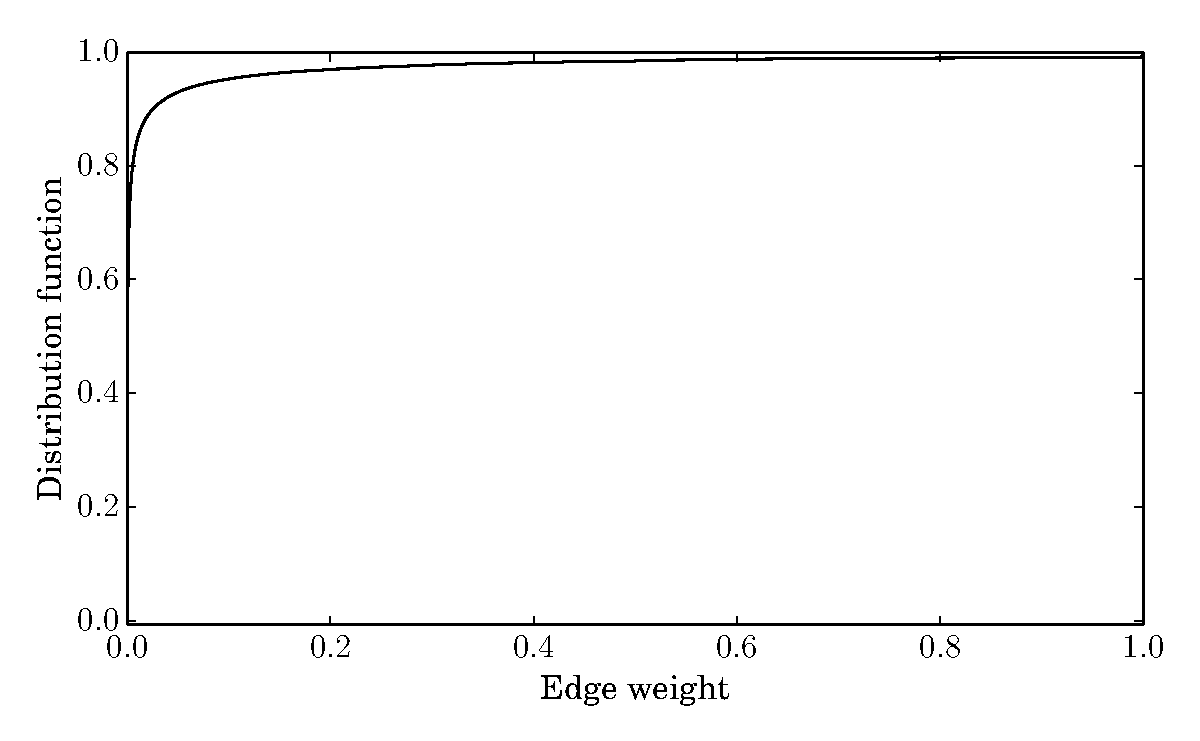
\includegraphics[width=0.75\columnwidth]{figures/billion-ew-cdf.pdf}}
\caption{The cumulative distribution function of edge weights in the Billion word correlation graph described in 
Sec.\ \ref{sec:words} shows that a large fraction of edges with low weights can be pruned. For example, 
approximately 90\% of the edges are discarded when considering edges with weights $\geq 0.01$.}
\label{fig:billion-ew-cdf}
\end{figure}

\begin{figure}
\centerline{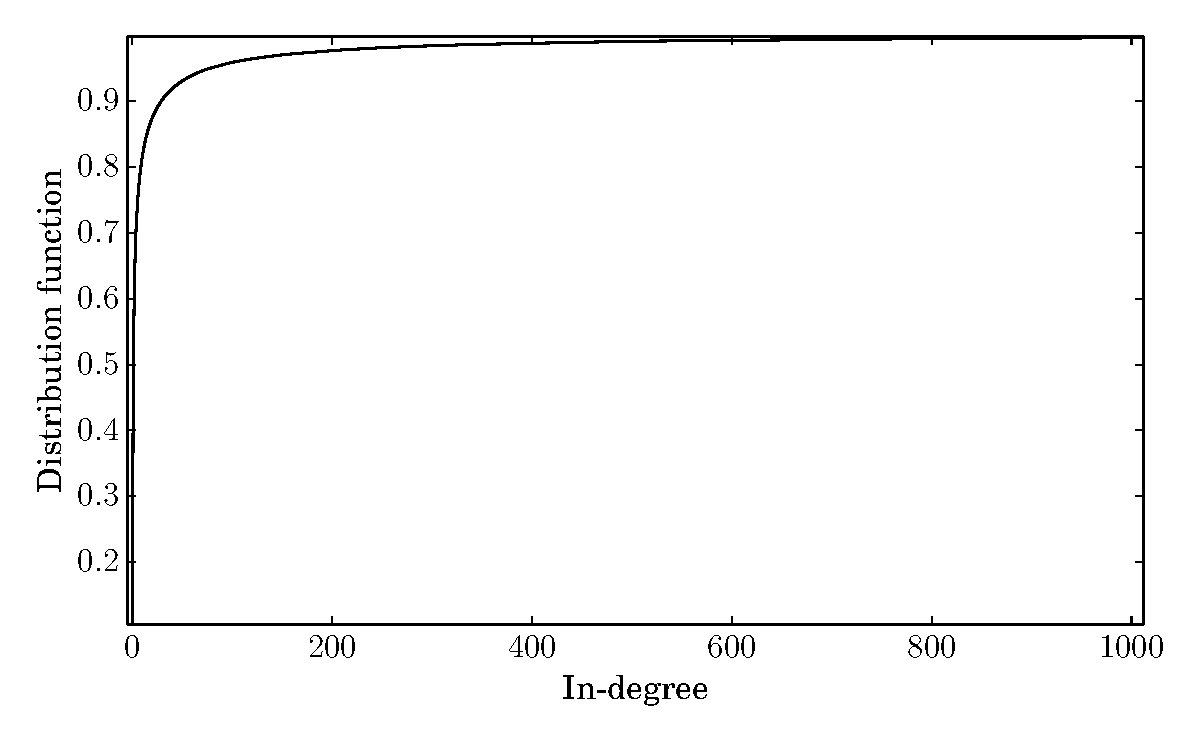
\includegraphics[width=0.75\columnwidth]{figures/billion-id-cdf.pdf}}
\caption{The cumulative distribution function of in-degrees for the graph referred to in Fig.\ \ref{fig:billion-ew-cdf}
 illustrates that it is possible to apply an in-degree threshold while affecting comparably few vertices. Only a small percentage
  of the vertices are affected, for instance, when capping the in-degree at 500 edges.}
\label{fig:billion-id-cdf}
\end{figure}

\subsection{Discovering concepts}
\label{sec:discoveringConcepts}

After transforming a correlation graph to a similarity graph, we can use the latter to find interesting
structural properties among objects in terms of their similarity relations. Since two objects are similar
if they occur in similar contexts, we can interpret the notion of \emph{similarity} as something that
the objects together exhibit if they are approximately exchangeable in their respective contexts,
being able to take each other's role. This notion of similarity  
requires very little, if any, assumptions about the properties of the objects \emph{per se}, since it is 
completely based on the relations \emph{between} objects.

Given a set of objects and their similarities, we can view a pair of objects $i$ and $j$ that have similarity
$\sigma_{i,j} = 1$ as equivalent. This is an equivalence relation in the formal sense
since it satisfies reflexivity, symmetry and transitivity. We can therefore partition the set of objects into
equivalence classes and interpret each class, in which all objects are interchangeable, as a concept.
Due to noise and slight variations, however, full similarity is seldom fulfilled in practical applications.
We therefore allow objects that are approximately similar,
i.e.~$\sigma_{i,j} \geq 1-\epsilon$ for some small constant $\epsilon$,
to belong to the same class. Due to this approximation, transitivity no longer holds, since although $i$ is approximately
similar to $j$ and $j$ is approximately similar to $k$, $i$ is not necessarily approximately similar to $k$.
From this follows that classes can overlap, which reflects that objects indeed may take several different roles
(consider for instance proteins with multiple functions, or polysemous words \cite{Palla2005}). 
Each concept is then constituted by a group of objects where each object has at least similarity $1-\epsilon$ to each other object. 

From a graph perspective, these
groups correspond to cliques (i.e.~complete subgraphs) in a similarity graph where $\sigma_{i,j} \geq 1-\epsilon$
for all edges. Since cliques can contain other cliques -- in fact, there is a combinatorial
explosion of such sub-cliques -- we require that a concept is a clique that is not a subset of another clique,
i.e.~it is a \emph{maximal clique}. However, finding maximal cliques in graphs is a highly challenging problem, both in theory
and practice. 
%There are several algorithms presented in the literature (see e.g.~\cite{}),
%but, to our knowledge, none of these are sufficiently efficient for our purposes. 
For this reason,
we approximate maximal cliques with \emph{communities}, i.e.~clusters of vertices in the similarity graph. 
An approach for finding such communities at scale is described in Sec.~\ref{sec:slpa-implementation}.

\subsection{Implementation}
\label{sec:algorithmsAndImplementation}

\subsubsection{Similarities}
\label{sec:similarity-implementation}

\begin{figure*}
\begin{lstlisting}
1: ins   = edges.map(((i,j),rij) => (j,(i,rij)))
2: pairs = ins.join(ins).filter((k,((i,rik),(j,rjk))) => i<j)
3: terms = pairs.map((k,((i,rik),(j,rjk))) => 
4:                   ((i,j),abs(rik-rjk)-abs(rik)-abs(rjk)))
5:              .reducebykey((v,w) => v+w)
\end{lstlisting}
\caption{Pseudo-code of the sum term calculation in Eq.\ \ref{eq:l1terms}. 1) Edge tuples with vertex indices \texttt{i} and
 \texttt{j}, and weights \texttt{rij} are mapped to key-value pairs keyed by destination vertices. 2) A two-hop graph is 
 generated through self-join, and unique in-edge pairs are extracted through filtering. 3-4) All terms in the sum in 
 Eq.\ \ref{eq:l1terms} are calculated and 5) summed per two-hop neighbour pair.
}
\label{fig:pseudocode}
\end{figure*}

The calculations of the approximations of the difference norms
$\dnm{i}{j}$, as formulated in Eq. \ref{eq:l1terms}, lend themselves well to functional
programming, since they can be implemented as a small number of standard transformations applied
on a collection of correlation graph edges. The procedure can be summarized in the following
steps:
\begin{enumerate}
\item For each vertex $i$, calculate the norms $\rns{i}$, i.e.~the weight sum prior
to pruning.
\item Prune the correlation graph by filtering out edges with weights below a given threshold value, $\mrn{i}$, and/or 
by keeping a given number of incoming edges with the largest weights per vertex.
\item Calculate $\tilde{\Lambda}_{i,j}$ for each pair of vertices that share at least one neighbour in the pruned correlation graph.
This step is described in pseudo-code in Fig.\ \ref{fig:pseudocode} and
involves a self-join operation for building a two-hop multigraph that links
second-order neighbours, followed by a map transformation for calculating the
terms in the sum, which subsequently are summed up per vertex pair by a reduce
operation.
\item For each vertex pair in the previous step, calculate the
approximate relative $L_1$-norm, $\tilde{l}_{i,j} =
(\tilde{\Lambda}_{i,j} + \psi_{i,j})/\psi_{i,j}$,
and  the approximate
similarity $\asy{i,j} = 1 - \tilde{l}_{i,j}$.
\end{enumerate}
The method is implemented in the Scala programming language and uses the in-memory
data processing framework Apache Spark \cite{Zaharia-2012}, which enables us
to employ the method at scale in terms of computing hardware.
To facilitate reproducibility, the implementation will be made available
with an open source license in an online repository.\footnote{https://github.com/sics-dna/concepts}
 Since we are exclusively using standard core primitives in Spark (\texttt{map},
\texttt{filter}, \texttt{join} etc.), implementing the
method in other similar frameworks, such as Apache Flink \cite{Alexandrov14}, is also
possible.

\subsubsection{Concepts}
\label{sec:slpa-implementation}
In order to find object clusters in the similarity graph, as previously mentioned, we employ a \emph{community detection} 
method (\emph{community} and \emph{cluster} are used interchangeably from here on). 
There is a wealth of techniques to choose from and we refer the reader to \citeasnoun{Fortunato2010}
for a thorough review of the area. For our purposes we need an algorithm that allows for overlapping communities
and has good scalability characteristics. The ability to detect overlapping communities is important for
concept discovery, as objects may exhibit multiple roles within a graph. 
Another preference is that the algorithm does not require that the 
number of clusters is predefined, but this number should rather be discovered from data.

Based on these criteria, we employ an algorithm that is akin to the Speaker-listener
label propagation algorithm (SLPA) by \citeasnoun{Xie2011}. In their algorithm, each vertex is assigned
a \emph{memory}, constituted by cluster label-frequency pairs, that is initialized with a unique cluster label. Vertices
are then updated sequentially and asynchronously: For a vertex $i$, each of $i$:s neighbours randomly 
(proportionally to label frequencies) sample a cluster label from their respective memories. These labels are then
sent to $i$, which adds the most common label to its memory. The procedure is repeated for a given number of 
iterations, after which vertices are assigned to clusters with frequencies above a specific threshold. 

In our implementation, all vertices are updated synchronously and in parallel, and instead of using
memories with frequency information, we associate each vertex with a \emph{queue} (i.e.\ a ``first in-first out" data type)
of community labels. More specifically, for each vertex $i$,
\begin{enumerate}
\item Initialize a queue $q_i = [i]$.
\item \label{start-of-loop} Sample a label uniformly from $q_i$ and send it to all neighbours.
\item \label{add-label} Of the received labels, add the one occurring most times to $q_i$. If $q_i$ has reached a maximum 
capacity, $\gamma$, discard the oldest label in $q_i$ prior to adding the new one. 
\item Repeat from step \ref{start-of-loop} $m$ times.
\item Associate $i$ with clusters with labels that occur in $q_i$ with a frequency above a given threshold.
\end{enumerate}
Since a vertex can be associated with several communities, the communities can overlap, including
the case where a community is a subset of another community. It is also possible that several equivalent clusters
are found, in which case the redundant ones are removed in a post-processing step.

The reason for storing cluster labels in queues, besides from ease of implementation, is that it has the effect 
that transient cluster assignments at early iterations are quickly discarded. 

Note that the current implementation does not take edge weights into consideration. Instead, edges with
weights below a threshold, $\sigma_m$, are discarded prior to applying the above steps. Generalizing the algorithm 
to support weights more gracefully is possible though, presumably, for instance, by weighting incoming cluster 
labels -- step \ref{add-label}  above -- with the weights of the edges with which the labels are communicated, prior to updating the queues.

\subsection{Scalability characteristics}
\label{sec:scalability-theory}
In order to enable practical use on large tasks in terms of the number of objects, correlations and example data,
a key design goal is scalability. Since we are using
relational primitives to represent graphs,
the scalability of the algorithm can be studied using established results from
relational algebra \cite{Chandra77,Bitton83}. 

The most computationally demanding component of the algorithm is
building the two-hop graph through a self-join operation (the third step in Sec.\ \ref{sec:similarity-implementation}).
Since a self-join is a conjunctive query \cite{Chandra77} in relational algebra terms,
we can reason about its computational cost.
Specifically for a distributed environment, \citeasnoun{koutris2011conjuctive}
define a parallel algorithm as a sequence of parallel computation steps, and define its
cost as the number of steps required to complete the algorithm.
The authors prove that a join operation can be completed in one parallel computational
step using the hash-join algorithm, by using a communication and a computation phase.
Just as importantly, they prove that the hash-join operation is load balanced
and as such it ensures linear speedup (doubling the server count reduces the load by
half) and constant scale-up (when doubling both the size of the data and number of servers, the running time remains the same).
Specifically for the Apache Spark platform, on which we implement the algorithm,
the self-join operation creates what \citeasnoun{Zaharia-2012}
call a \textit{narrow dependency}. This property allows for pipelined executions
of all operations on one node up until the reduction step in Fig. \ref{fig:pseudocode}, without the need for expensive data shuffles
through the network.

\section{Experiments}
\label{sec:experiments}

\subsection{Examples}
In order to demonstrate the broad applicability of our approach, we will showcase it in three distinct 
domains: computational linguistics, music and molecular biology. Here we prioritize breadth over depth, and more in-depth evaluations 
of the method's performance with respect to specific applications will be topics in future work.

\subsubsection{Words}
\label{sec:words}

\begin{figure*}
\centerline{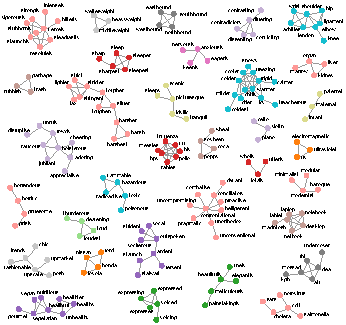
\includegraphics[width=1.0\columnwidth]{figures/billion-words-example.pdf}}
\caption{Examples of groups of words in a word similarity graph based on the Billion word corpus. 
For sake of clarity, edges with weights $\sy{i,j} \geq 0.15$ are shown.}
\label{fig:billion-words-example}
\end{figure*}

We begin by relating words in terms of their co-occurrence in text, where two words, $i$ and $j$, co-occur if they both
appear within a window of $n$ words. In the simplest case, for $n = 2$, words co-occur if they are adjacent.
There exist many different word association measures, see \cite{Pecina08} for a large number of examples, such as
pointwise mutual information \cite{Church90} and normalized versions thereof \cite{Bouma09}. Here we simply measure the
association between $i$ and $j$ as the relative frequency of $j$ occurring in $i$:s vicinity, or, in other words, as the
conditional probability that a randomly selected word in a window that contains $i$, will be the word $j$. That is, $\rn{i,j}
\approx c_{i,j}/{c_i}$, where $c_i$ and $c_{i,j}$ are the number of occurrences of $i$, and $i$ together with $j$,
respectively. Note that this measure is not symmetric and so $\rn{i,j} \neq \rn{j,i}$ may be true.

The method is applied on two datasets: the One billion word \cite{Chelba13} and
the Google Books n-gram \cite{Michel10,Lin12} datasets. The former consists of
nearly one billion tokens and originates from crawled online news texts. From
these we count the number of occurrences of bigrams (pairs of adjacent words) with words consisting only
of alphabetic characters. This results in approximately 8 million unique
bigrams and a vocabulary with roughly 0.3 million words. From the bigram counts
we relate words by their ordered adjacency.

Despite the comparably modest size of this corpus and the narrow context window, the method
manages to discover groups of words that reflect both syntactic and semantic
concepts. Examples of such concepts are shown in Fig.\ \ref{fig:billion-words-example},
where we see that the groups correspond e.g.\ to specific nouns,
 (\emph{tablet}, \emph{laptop}, \emph{notebook} etc.), adjectives
 (\emph{chic}, \emph{trendy}, \emph{fashionable} etc.), or adverbs
 (\emph{strongly}, \emph{intensely}, \emph{vigorously}, etc.). Note that antonyms, in addition to synonyms, 
 may occur in the same group (e.g. \emph{warmer} and \emph{colder}). This highlights that the notion of similarity (here
 corresponding to what is termed \emph{relatedness} in the NLP field)
 is very much dependent on the choice of correlation measure. The correlation measure may therefore be both
 application and domain-specific, whereas the definition of similarity, \emph{given} the correlation measure, is domain-agnostic. 
 Accordingly, antonyms are indeed similar by definition with respect to the correlation measure used in this example. However, 
 for other correlation measures, possibly supporting negative correlations, antonyms may occur in separate concepts.

The Google Books n-gram dataset, which consists of 361
billion tokens for the English language version of the dataset, is used both to evaluate the scalability of the
method, which will be discussed in Sec.\ \ref{sec: scalability}, and to quantify the quality of resulting similarity
relations. An n-gram can be defined as a contiguous sequence of $n$ words in a text.
To further challenge the method, we apply it on correlation graphs with respect to co-occurrence
windows of size 5. This results in a denser correlation graph, since a
word has more neighbors due to the larger co-occurrence window size. Nevertheless, the
key properties that we describe in Sec.\ \ref{sec:approximations} still
apply and we can prune away a large number of edges with low weights.

A common approach to quantitatively evaluate the performance of word association methods is to use benchmarks
with word pairs that have been manually graded with respect to degree of association. Since these
benchmarks also contain unassociated words, it is not possible to do a direct comparison between our
method and other
approaches in terms of benchmark performance, since our method exclusively relates words that have a certain
degree of similarity (indeed, this is one of the reasons it is scalable). However, to give an indication of
the method's performance, we measure the Spearman rank correlation coefficient between benchmark
similarities and $\sy{i,j}$ for word pairs $(i, j)$ that \emph{do} exist in the similarity graph. For this purpose we
use the standard WS-353 test collection \cite{Finkelstein01}, which consists of 353 word pairs that have
been graded by human annotators. We build a similarity graph from co-occurrence windows of size 5, filter
out words that occur with a frequency less than $10^{-8}$ and edges $\rn{i,j} < 10^{-3}$, and
set the maximum in-degree to 200. In this graph, which is built in less than 10 minutes (cf. Fig.\ \ref{fig:google-e-runtime}),
60\% of the WS-353 word pairs are present, resulting in a Spearman rank correlation of 0.76. The current state of the
art (with respect to the whole dataset) is 0.81 \cite{Halawi12,Yih12}.
These figures represent the correlation with respect to the average annotator score. Note, however,
that there is low inter-annotator agreement in WS-353, where the mean performance
of individual annotators, with respect to the mean score of the remaining annotators, is in fact also 0.76 \cite{Hill14}.

\subsubsection{Artists}
In the next proof-of-concept we relate artists by using a dataset that represents the listening
habits of users of the \emph{Last.fm} music service.\footnote{http://www.last.fm/} This dataset, provided by
\citeasnoun{Celma2010}, consists of approximately 19 million track plays of 992 users. For each user, we extract sequences of
played artists -- there are roughly 177000 in total -- and consider the context of an artist to be defined by the probability
distribution of subsequently played artists. Hence, we assume artists are related in a Markov chain, where each artist
constitutes a state, and where there is a directed edge from artist $i$ to artist $j$ weighted with the probability
that $j$ is played next, given that $i$ is currently playing. This probability is simply estimated as $\rn{i,j} \approx
c_{i,j}/c_i$, where $c_i$ and $c_{i,j}$ are the number of times $i$, and $i$ followed by $j$ occur in the data set,
respectively.

The in-degree distribution of the artist correlation graph resembles those of the word correlation graphs,
which again means that relatively few vertices are affected by in-degree pruning. Transforming the artist correlation
graph to a similarity graph also results in tightly grouped artists that can be clustered, where the resulting
clusters appear to represent musical genres as exemplified in Fig.\ \ref{fig:artists}. As such, the similarity graph could
 be used in a music recommendation system to relate similar artists 
through the listening habits of users, similar to a collaborative filtering system. We could then also provide an
 intuitive way to incorporate the popularity of artists via their play frequencies in order to mitigate the 
 effect of popularity bias in recommendations \cite{celma2008hits}.

\begin{figure}
\centerline{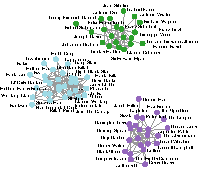
\includegraphics[width=0.75\columnwidth]{figures/last-fm-example-3.pdf}}
\caption{Examples of components in an artist similarity graph correspond to three distinct music genres. Edges with weights $\sy{i,j} \geq 0.5$ are shown.}
\label{fig:artists}
\end{figure}

\subsubsection{Codons}

Finally, we apply the method in molecular biology, where we consider codons as objects. Codons are triplets of
adjacent nucleotides in DNA that translate to amino acid residues that in turn form proteins.  These are related
through codon substitution dynamics, which is central both for understanding molecular evolution and in applications
such as DNA sequence alignment \cite{Anisimova09}. Since there are only 64 codons in total, this example differs from
the previous two in that we consider relatively few objects.

Codon substitutions are often modeled as Markov processes \cite{Anisimova09}, where the
substitution probabilities of a codon at a specific location are assumed to be independent of neighbouring codons as
well as previous codons at the same location. In this example we use an empirically derived codon substitution matrix 
provided by \citeasnoun{Schneider2005}, where we consider the context of a codon $i$ to be given by the relative substitution frequencies
$(\rn{i,j})_{j=1}^n$ to other codons $j$.

\begin{figure}
\centerline{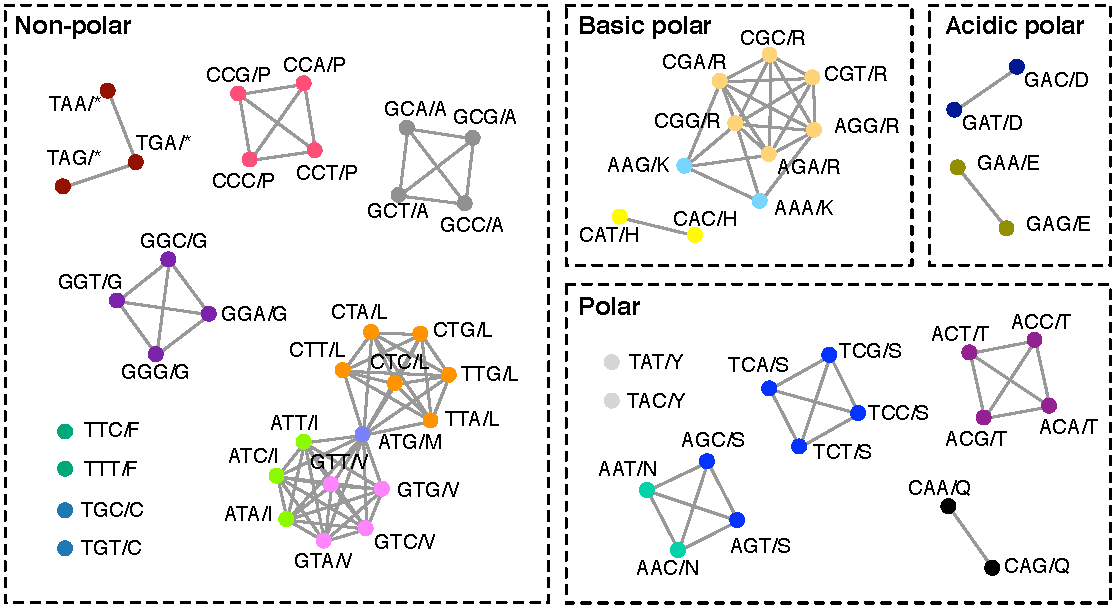
\includegraphics[width=0.9\columnwidth]{figures/codon-example.pdf}}
\caption{Codon similarity graph where vertices are labeled with $c/a$ for codon $c$ coding to amino acid $a$. Edges
with weights $\sy{i,j} \geq 0.45$ are shown. Vertices are color coded with respect to amino acids and grouped by
chemical properties. Note that when the edge weight threshold is lowered, clusters containing several amino acids are split by
amino acid. The rare and low mutable amino acid tryptophan is omitted. }
\label{fig:codons}
\end{figure}

As seen in the resulting codon similarity graph in Fig.\ \ref{fig:codons}, codons that translate to the same amino acid according
to the standard genetic code \cite{Nirenberg65} tend to be grouped. This reflects that codons that are highly similar
are commutable -- quite literary -- since substitutions between these codons are neutral under evolution. These clusters are also
present in the correlation graph and therefore preserved through the similarity graph transformation.

We now shift perspective and view \emph{amino acid} as a concept. Again looking at Fig.\ \ref{fig:codons},
we see that some of the amino acids are grouped. This can be explained by a higher degree of neutrality within groups
than between them, which has been observed in empirical amino acid substitution matrices, such as the accepted point
mutation (PAM) matrix by Dayhoff et al. \cite{Dayhoff78}. In comparison, Wu and Brutlag derived amino acid substitution
groups by group-wise (as opposed to pairwise) statistical analysis of protein databases \cite{Wu96}.  The groups shown
in Fig.\ \ref{fig:codons} (\{I, L, M, V\}, \{K, R\} and \{N, S\}) all agree with their findings. In summary, the codon similarity 
graph captures both concepts and higher-order concepts: from codons to amino acids, via the genetic code,
to collections of amino acids that constitute known substitution groups.

\subsection{Concept discovery}
\begin{figure}
\centerline{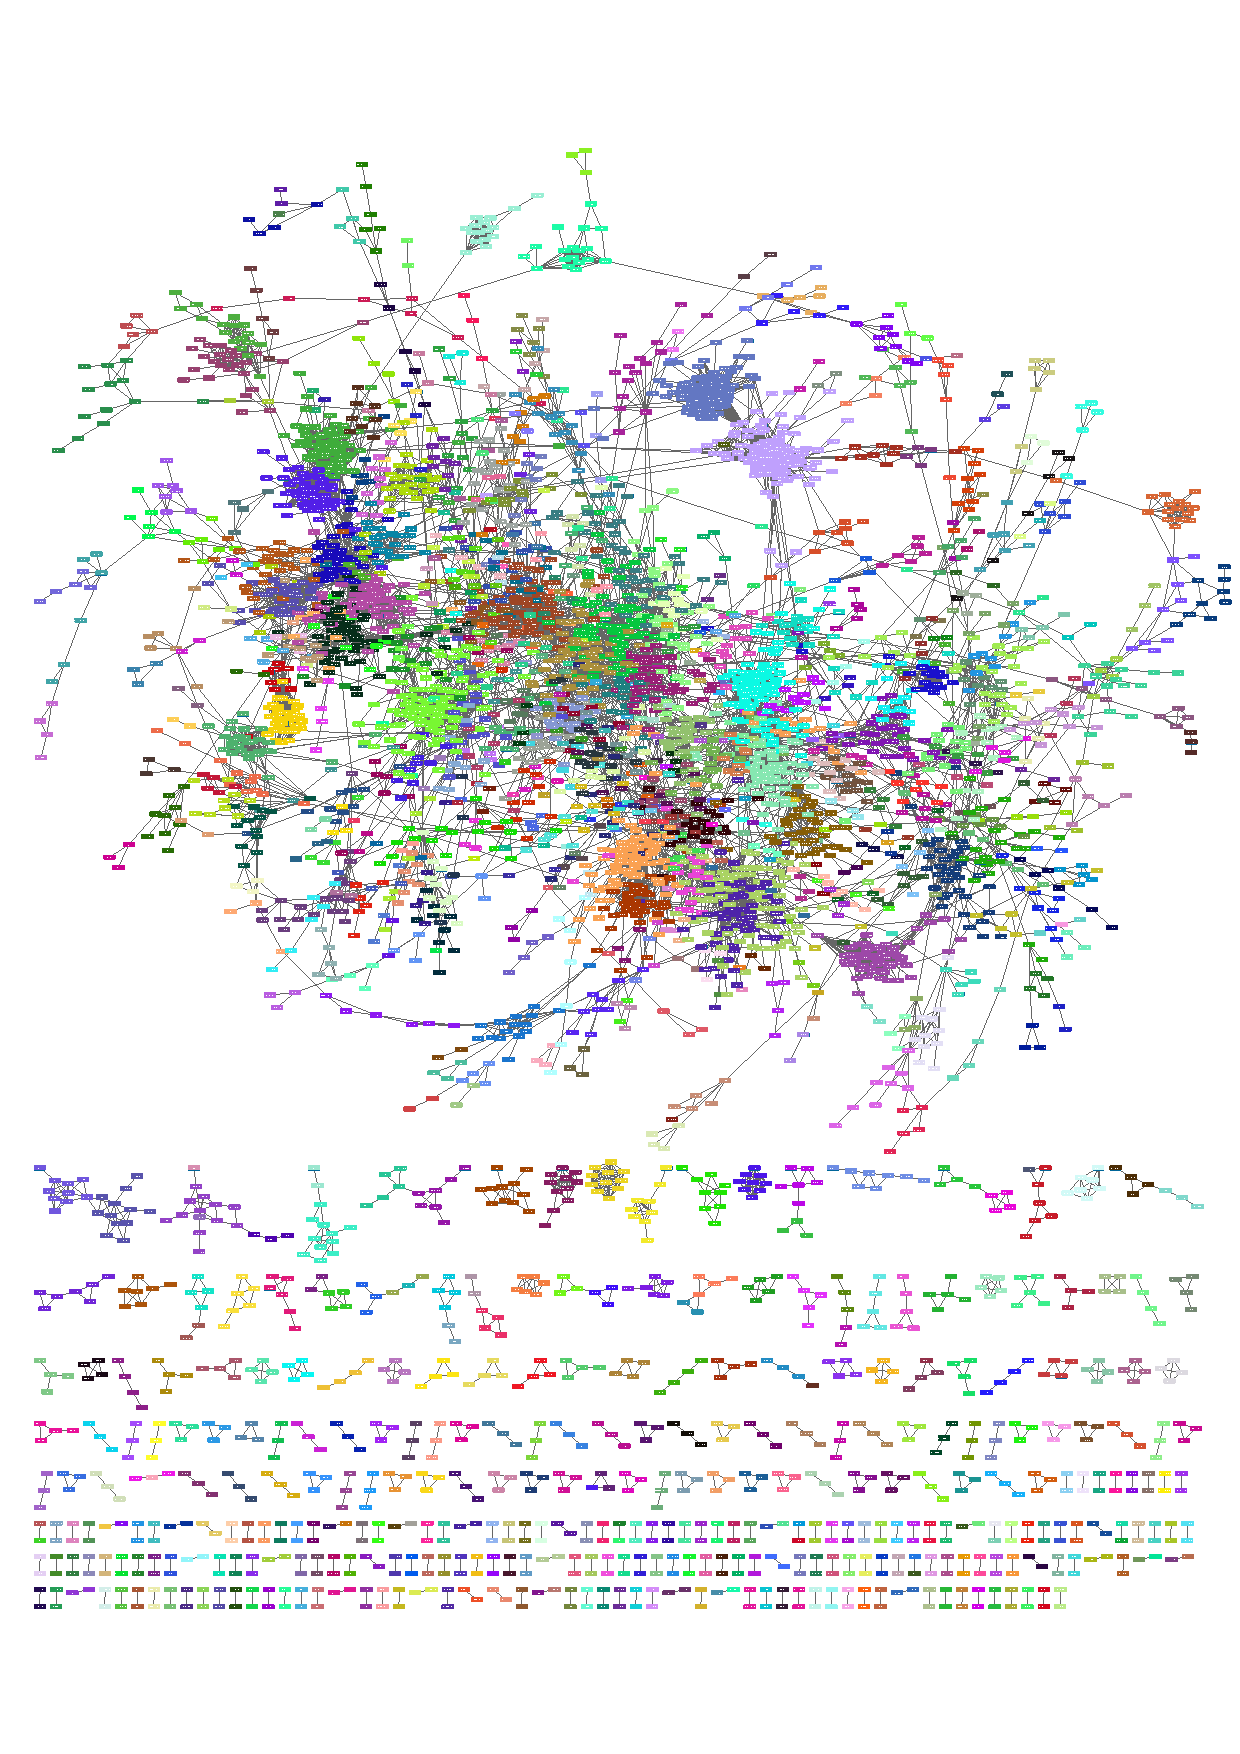
\includegraphics[width=1.0\columnwidth]{figures/slpa-complete-adjusted_cropped.pdf}}
\caption{Similarity graph color coded by concept (vertex labels are visible after zooming the figure in the electronic 
version of the paper). The visualization is done with \emph{Cytoscape} \protect\cite{Shannon2003}.}
\label{fig:graph-overview}
\end{figure}

\begin{table}
\caption{Uniformly sampled examples of concepts.}
\begin{center}
\renewcommand{\arraystretch}{1.3}
\begin{tabular*}{\textwidth}{l|l}
\hline
achievements, examples &
minority, majority \\
\hline
burning, burn & 
founding, associate \\
\hline
breakfast, lunch &
thinking, thought \\
\hline
removing, remove &
foreign, overseas\\
\hline
easy, easier &
chrysler, inc\\
\hline
colour, color &
found, discovered, bodies\\
\hline
loved, liked, enjoy, loves &
heard, hear, hearing\\
\hline
liquid, toxic &
fiscal, banking, financial, economic, gambling\\
\hline
tuition, tax &
solar, wind\\
\hline
britain, nation &
impose, enforce, violating, violated, imposed, imposing\\
\hline
\end{tabular*}
\end{center}
\label{table:random-clusters}
\end{table}

\begin{table}
\caption{Selected examples of concepts.}
\begin{center}
\renewcommand{\arraystretch}{1.3}
\begin{tabular*}{\textwidth}{p{\textwidth-0.3cm}}
\hline
significant, dramatic, greater, major, enormous, modest, substantial, incredible, sharp, slight, 
considerable, meaningful, largest, greatest, tremendous, biggest, bigger, great, unprecedented, 
sudden, huge, rapid, steady, vast, massive, big, genuine, large \\
\hline
dallas, memphis, milwaukee, pittsburgh, detroit, cincinnati, indianapolis, diego, sydney, la, 
houston, cleveland, chicago, louis, sacramento, oakland, orleans, vancouver, francisco, 
orlando, angeles, baltimore, seattle, philadelphia, phoenix, buffalo, columbus, atlanta, vegas, denver, boston, montreal, toronto, miami, portland\\
\hline
yale, harvard, duke, oxford, cambridge, school, ucla, stanford, university, college \\
\hline
arkansas, colorado, jersey, delaware, georgia, kansas, florida, mississippi, minnesota, 
wisconsin, dakota, massachusetts, indiana, california, maine, pennsylvania, illinois, utah, 
carolina, louisiana, alaska, tennessee, texas, missouri, maryland, oklahoma, iowa, 
montana, hampshire, oregon, nevada, kentucky, ohio, alabama, connecticut, michigan, virginia, arizona\\
\hline
grey, white, yellow, gray, blue, pink, red, dark, orange, black, green\\ 
\hline
van, convoy, vessel, aircraft, ship, bus, boat, crews, vessels, cycle, bike, vehicle, trains, 
boats, helicopters, ships, vehicles, jet, helicopter, truck, buses, car, cars, flights, planes, 
firefighters, motorcycle, trucks, plane\\ 
\hline
telegraph, tribune, post, xinhua, times, magazine, newspaper, mirror, observer, herald, 
guardian\\
\hline
broadcasting, mining, banking, tech, telecommunications, wholesale, utility, retail,
 telecom, infrastructure\\ 
\hline
main, principal, key, decisive, vital, precious, helpful, valuable, critical, useful, essential, 
crucial, necessary, important\\ 
\hline
appears, sounds, appeared, sound, seemingly, looks, appear, seem, seems, appearing\\ 
\hline
soccer, tennis, diving, nba, cycling, boxing, hockey, sailing, basketball, football, baseball, 
rugby, nfl, golf, cricket, nhl, swimming\\
\hline
weeks, years, year, days, month, quarters, hours, hour, contests, moments, decades, 
holes, centuries, week, months, shortly, primaries, decade, minutes, seconds\\
\hline
tomorrow, wednesday, sunday, today, yesterday, monday, thursday, tuesday, tonight, 
saturday, friday\\
\hline
footage, photograph, season, images, episode, pictures, episodes, videos, photographs, 
tape, sessions, session, photos\\
\hline
high, lower, highest, upper, lowest, average, low, median, higher\\
\hline
gold, fuel, ore, electricity, silver, copper, water, ethanol, petroleum, oil, gas, uranium, 
coal, power, energy, petrol\\
\hline
isolated, remote, wealthy, urban, vulnerable, poor, poorer, poorest, impoverished, rural\\
\hline
ninth, third, first, sixth, fourth, fifth, seventh, second, eighth\\
\hline
venezuelan, british, italian, australian, palestinian, american, spanish, iranian, yemeni, afghan, 
georgian, swedish, austrian, lankan, lebanese, irish, german, argentine, saudi, indian, brazilian, 
greek, dutch, serbian, communist, egyptian, cuban, myanmar, pakistani, israeli, colombian, 
nigerian, tibetan, syrian, mexican, russian, portuguese, korean, somali, thai, soviet, swiss, us, 
czech, french, polish, chinese, uae, sudanese, japanese, belgian, norwegian, turkish, kurdish, 
tibet, indonesian, canadian, haitian, iraqi, english, danish, tamil\\
\hline
\end{tabular*}
\end{center}
\label{table:selected-clusters}
\end{table}

We will now demonstrate the concept discovery approach by applying the clustering algorithm described in 
Sec.~\ref{sec:slpa-implementation} on a similarity graph transformed from a word correlation graph.
The latter is again built from the Billion word corpus using bigram counts. However, correlations $\rn{i,j}$
are now given by the pointwise mutual information between $i$ and $j$ \cite{Church90}:
\begin{equation}
\rn{i,j} = \log_2 \frac{p_{i,j}}{p_i\ p_j},
\end{equation}
where $p_i$ and $p_j$ are the probabilities that $i$ and $j$ are observed in the corpus, and $p_{i,j}$ is the probability
that they are observed together (here meaning being adjacent). 
These probabilities are estimated by $p_i \approx c_i / c_{t}$, $p_j \approx c_j / c_{t}$ and
$p_{i,j} \approx c_{i,j} / c_{t}$, where $c_i$, $c_j$ and $c_{i,j}$ are occurrence counts, and where $c_{t}$ is the total number
of tokens in the corpus. Since $p_i\ p_j$ is the probability that $i$ and $j$ co-occur if they were independent, 
$\rn{i,j} = 0$ means that the objects are completely unrelated. If 
$i$ and $j$ co-occur more frequently than expected from chance, then $\rn{i,j} > 0$. Similarly, $\rn{i,j} < 0$ if they 
are observed together to a less extent than expected. Note further that the measure is symmetric, i.e.~$\rn{i,j} = \rn{j,i}$.
In comparison to associating objects with conditional probabilities,
pointwise mutual information has the advantage of being less dominated by very frequent object occurrences (consider for
instance the correlation between a relatively infrequent word and a word such as \emph{the}).

The correlation graph consists of vertices with $p_i \geq 10^{-5}$ and edges with $\rn{i,j} \geq 4$ bits, and has 
a maximum in-degree of 1000 edges. When clustering the corresponding similarity graph, 
$\sigma_m = 0.25$, queues have capacity 4, and the iteration described in \ref{sec:slpa-implementation} is performed 16 times. 
The resulting cluster assignments are then given by labels that occupy at least 50\% per queue. Out of these, the most 
dominant cluster assignments per vertex are depicted in Fig.~\ref{fig:graph-overview}.

As examples, a random set of clusters is shown in Table \ref{table:random-clusters}, and a set of clusters of our choosing in Table \ref{table:selected-clusters}. Both sets -- with some exceptions (e.g. \{britain, nation\}, perhaps due to that both
words are strongly correlated with \emph{great}) -- demonstrate that the method is capable of discovering 
concepts that we perceive as meaningful in that they capture abstract syntactic and semantic notions in the corpus, such as
\emph{vehicle}, \emph{US state} (which, incidentally, also demonstrates our bare-bones parsing of the corpus,
since \emph{carolina} and \emph{hampshire} -- lacking \emph{north}, \emph{south} and \emph{new} -- belong to this concept),
\emph{color}, \emph{nationality}, \emph{day} and so on.

\subsection{Accuracy}
\label{sec: accuracy}

\begin{figure}
\centerline{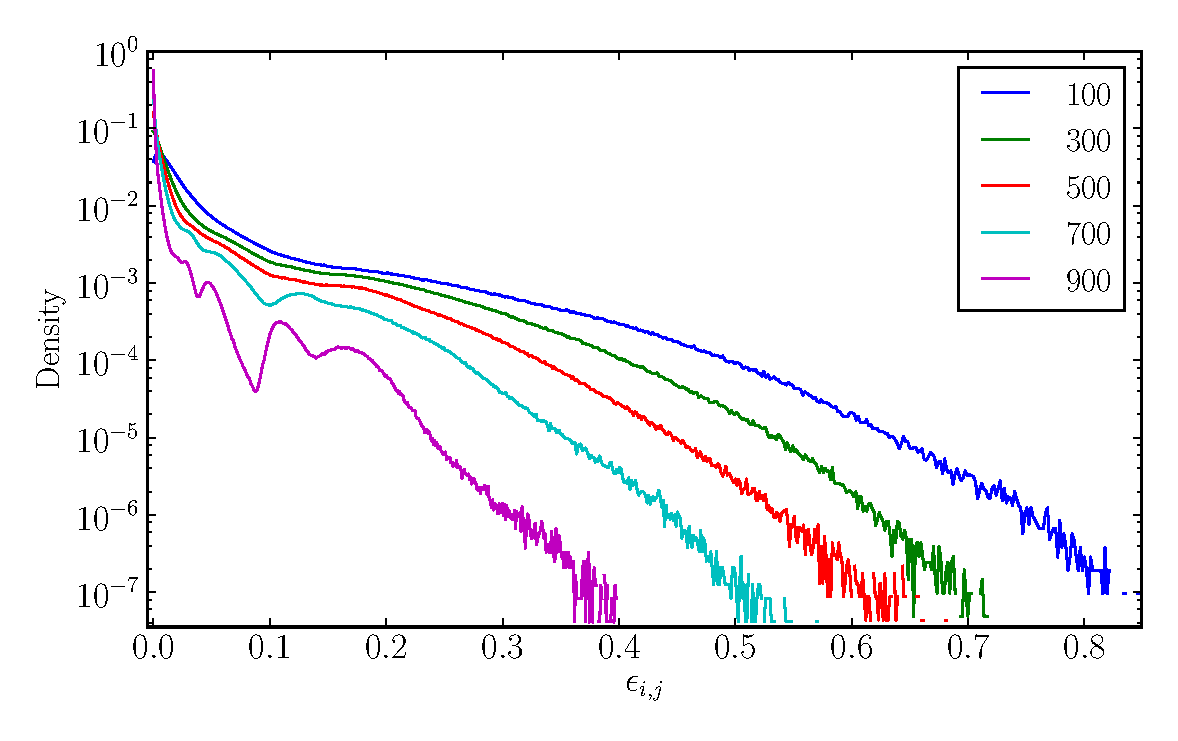
\includegraphics[width=0.75\columnwidth]{figures/1446451652-absolute_error.pdf}}
\caption{Densities of absolute similarity errors $\epsilon_{i,j}$ for different in-degree thresholds $\delta$.}
\label{fig:abs-error}
\end{figure}

\begin{figure}
\centerline{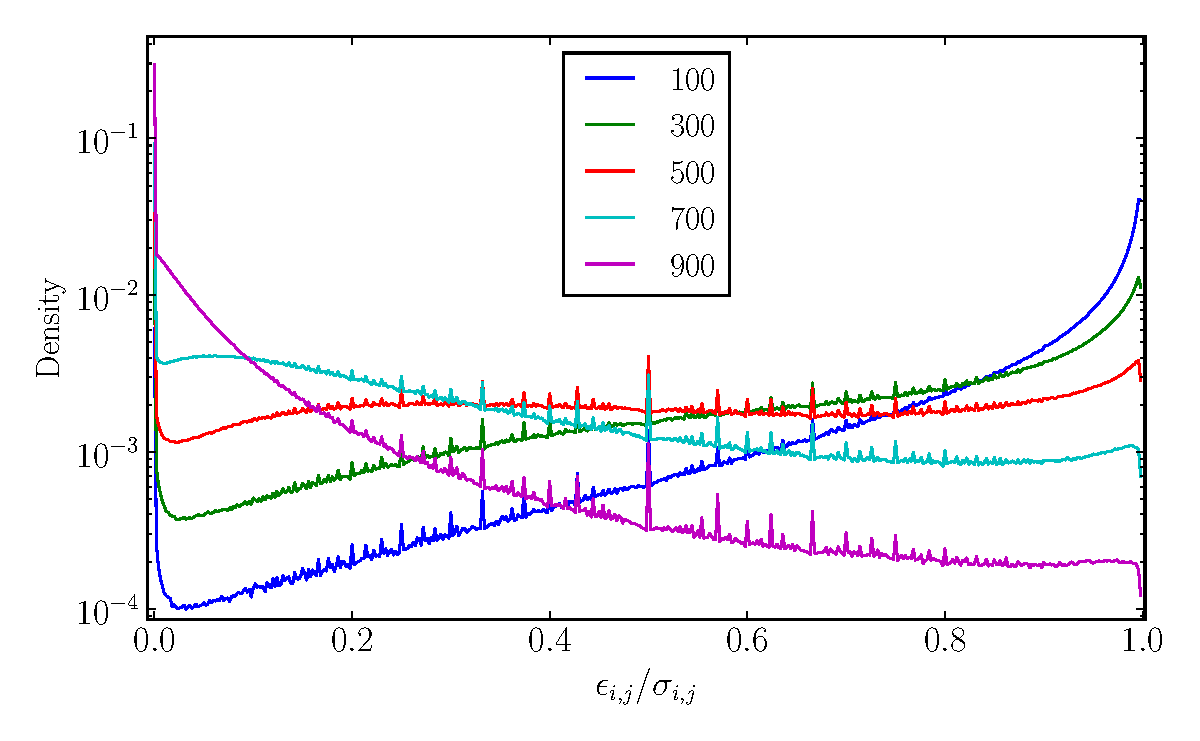
\includegraphics[width=0.75\columnwidth]{figures/1446451652-relative_error.pdf}}
\caption{Densities of relative similarity errors $\epsilon_{i,j}/\sigma_{i,j}$ for different 
in-degree thresholds $\delta$.}
\label{fig:rel-error}
\end{figure}

We evaluate the accuracy experimentally as follows:

\begin{enumerate}
\item Build a reference correlation graph $\mathcal{R}$ that constitutes the ground truth. 
Here $\mathcal{R}$ is built from co-occurrence frequencies in the Billion word corpus, 
where correlations are given by conditional probabilities as described in Sec.\ \ref{sec:words}.
Correlations where $\rho_{i,j} \geq 10^{-5}$ are kept and in-degrees are capped at 1000.
Furthermore, words occurring with a frequency less than $10^{-5}$ are discarded.
\item Transform $\mathcal{R}$ to a similarity graph $\mathcal{S}$, being the
\emph{true} similarity graph.
\item For different in-degree thresholds $\delta \in \{100, 300, ..., 900\}$:
\begin{enumerate}
\item Prune $\mathcal{R}$ into an approximate correlation graph $\mathcal{R}_{\delta}$.
\item Transform $\mathcal{R}_{\delta}$ into an approximate (with respect to $\mathcal{R}$) similarity 
graph $\mathcal{S}_{\delta}$. 
\item Calculate the errors $\epsilon_{i,j} = |\sigma_{i,j} - \tilde{\sigma}_{i,j}|$ as the differences between
the edge weights in corresponding edges $(i,j)$ in $\mathcal{S}$ and $\mathcal{S}_{\delta}$.
\end{enumerate}
\end{enumerate}

The result of this procedure is shown in Figures \ref{fig:abs-error} and \ref{fig:rel-error}, where we
plot the densities (normalized counts of binned errors) of the absolute error $\epsilon_{i,j}$, as well as of the relative error, 
$\epsilon_{i,j}/\sigma_{i,j}$ with respect to the similarity. In both cases the approximation
errors quickly decrease with growing in-degree thresholds. Note also that the relative error in 
Fig.\ \ref{fig:rel-error} is consistent with the error bound in Eq.\ \ref{eq:rel-error-bound} in being bound by 1.

We hypothesize that the relative errors tend to be smaller for large similarities $\sigma_{i,j}$ than for
 small ones, since if a correlation $\rho_{i,k}$ between $i$ and some $k$ is sufficiently small to be discarded,
the same goes for the correlation $\rho_{j,k}$  as $i$ and $j$ are similar. This has the effect that the number of
discarded terms in  $\Lambda_{i,j}$, cf.~Eq.~\ref{eq:error-prime}, is comparably small (the number 
of discarded terms is at most the sum of discarded edges of $i$ and $j$, which is the case when neither of these
edges share a common terminal $k$). To test this hypothesis, we plot a heat map (i.e., a color-coded 2-dimensional 
histogram) of the similarities $\sigma_{i,j}$ and the relative errors $\epsilon_{i,j}/\sigma_{i,j}$ (see Fig.\ \ref{fig:error-heatmap}), 
and indeed, the relative error appears to be negatively correlated with the similarity.

\begin{figure}
\centerline{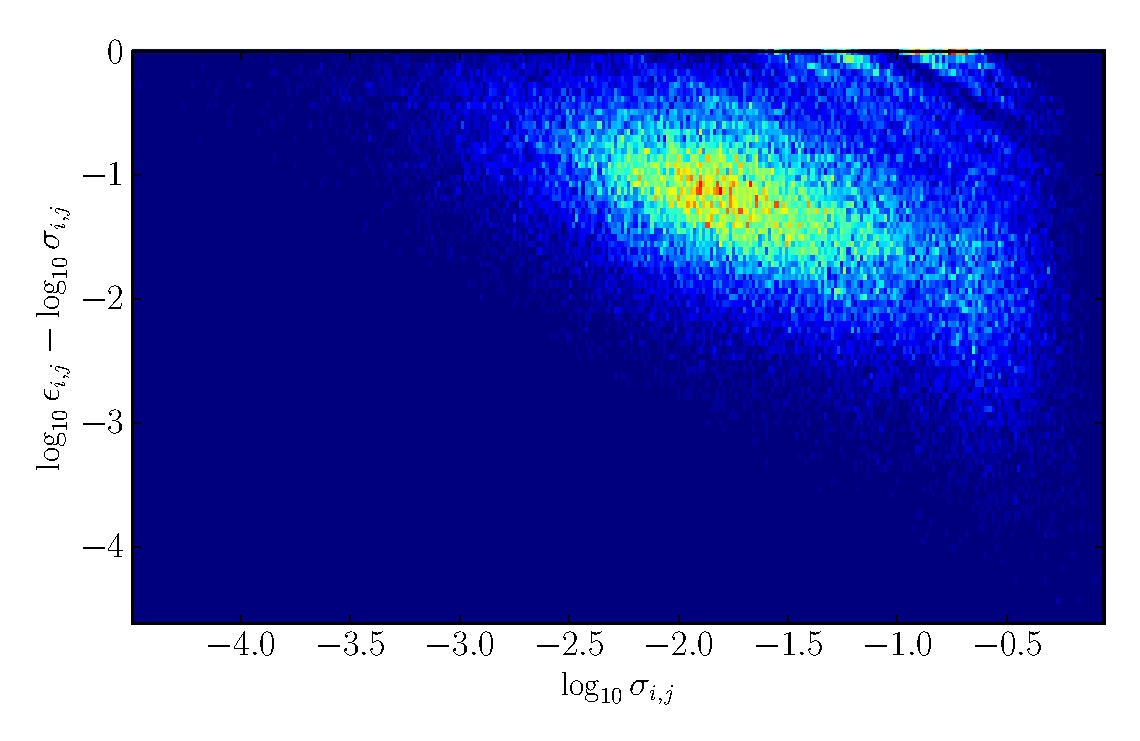
\includegraphics[width=0.75\columnwidth]{figures/1446451652-relative_error-heatmap-900.pdf}}
\caption{Heat map of similarities $\sigma_{i,j}$ and relative errors $\epsilon_{i,j}/\sigma_{i,j}$ (log scale)
for $\delta = 900$. Red, yellow and cyan indicate a high density, whereas blue indicates a low density.}
\label{fig:error-heatmap}
\end{figure}

\subsection{Scalability}
\label{sec: scalability}

\begin{figure}
\centerline{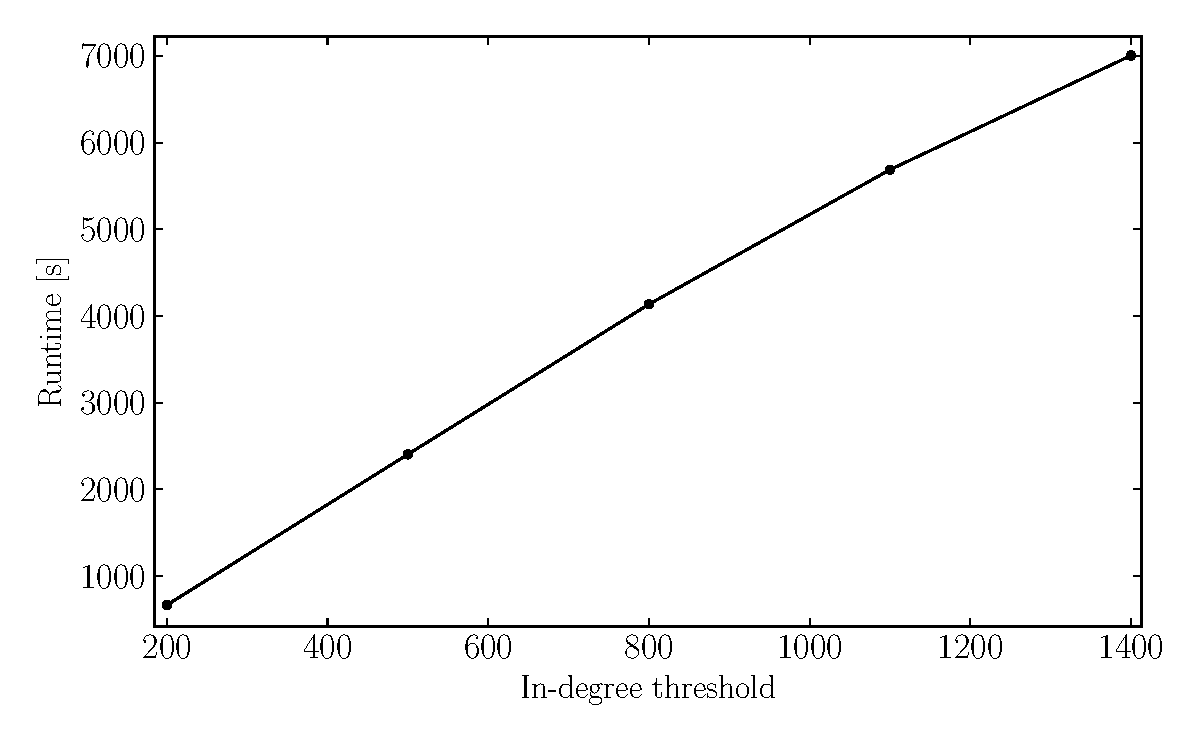
\includegraphics[width=0.75\columnwidth]{figures/billion-rt-2.pdf}}
\caption{Runtime for different in-degree 
thresholds, and $\rn{i,j} \geq 10^{-5}$. Built from bigrams in the One billion word corpus using a commodity laptop.}
\label{fig:billion-e-runtime}
\end{figure}

To demonstrate that our approach is applicable at scale in practice, we apply it on a dataset that is based on 
one of the largest, to our knowledge, text corpora currently available, the Google Books
n-gram dataset \cite{Michel10,Lin12}, which corresponds to approximately 4\% of all books ever printed.
The dataset is publicly available, and in our experiments we use
the version that is available through the Amazon S3 service.\footnote{https://aws.amazon.com/datasets/google-books-ngrams/}
As described in Sec.\ \ref{sec:words}, we use the English language corpus
which contains approximately 361 billion tokens. When processed into 5-grams, the corpus results in a file with 24.5 billion 
rows and the total compressed size of the dataset is 221.5 GB. This data is pre-processed to create the correlation graph by retaining
only alphabetic characters. The resulting correlation graph before pruning has 706,108 vertices and 94,945,991 edges.

To perform the experiments we employ an Apache Spark cluster created using the Amazon
Web Services EC2 service.\footnote{http://aws.amazon.com/ec2/}
The cluster consists of 8 nodes (1 master and 7 slaves), where each node has 4 vCPUs and
30.5 GiB of memory (EC2 instance type \emph{r3.xlarge}), such that the total amount of memory available to the cluster
is roughly 186 GiB, as reported by Spark.

\begin{figure}
\centerline{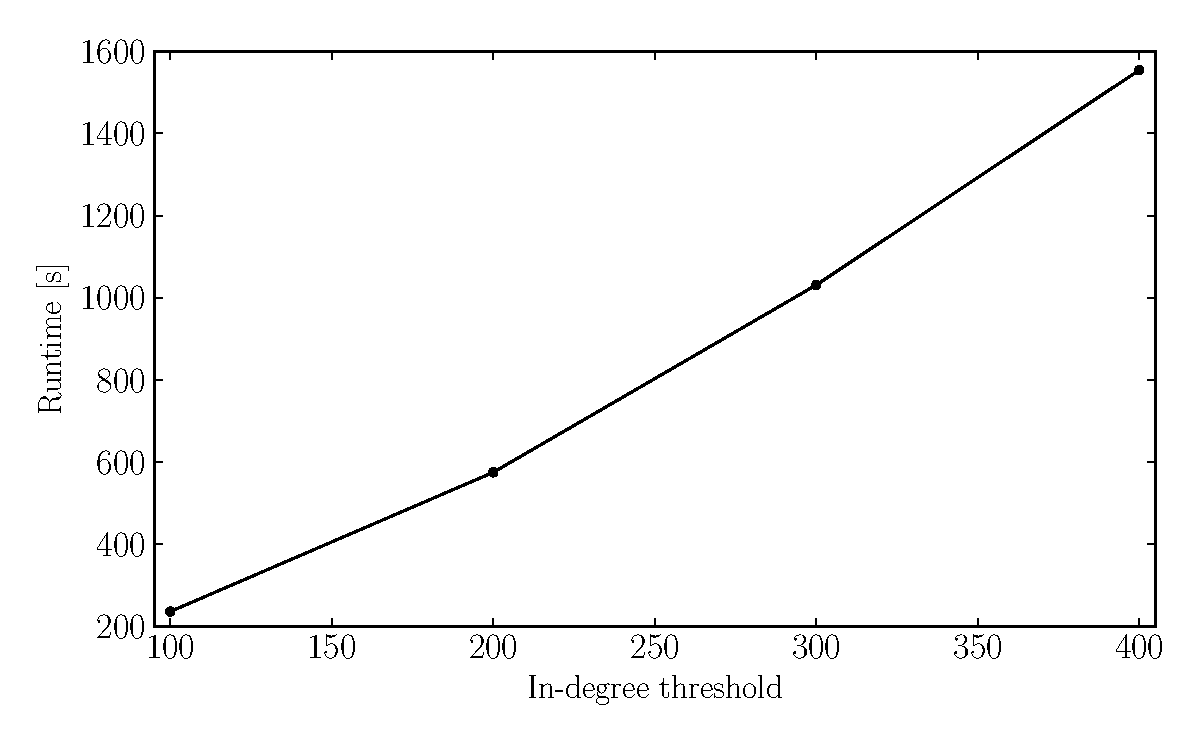
\includegraphics[width=0.75\columnwidth]{figures/eng-all-edge-low-e3-vtx-low-e8-high-e1-100-400-idg-nt.pdf}}
\caption{Runtime for different in-degree 
thresholds, and $\rn{i,j} \geq 10^{-3}$. Built from Google Books 5-grams using an Amazon
EC2 cluster (see text for details).}
\label{fig:google-e-runtime}
\end{figure}

The experiment results support the theoretical investigation of the computational
cost of the algorithm, cf.~Sec.~\ref{sec:scalability-theory}, and together with the pruning
described in Section \ref{sec:approximations} we are able to transform correlation graphs into similarity
graphs in reasonable amounts of time. This also holds true when using more modest computational resources,
as shown in Fig.\ \ref{fig:billion-e-runtime}, for building similarity graphs using the Billion word corpus as described
in Sec.\ \ref{sec:words}. Analogous results are achieved in the Google 5-gram case, here with runtimes on the order of minutes,
as seen in Fig.\ \ref{fig:google-e-runtime}. The experiments were replicated three times, and
the runtimes are reported in Table \ref{tab:google_runtimes}.
Together with Fig.\ \ref{fig:abs-error}, Fig.\ \ref{fig:billion-e-runtime} and Fig.\ \ref{fig:google-e-runtime} illustrate the trade-off between accuracy, controlled
via the in-degree threshold, and runtime, where the runtime scales favourably with an increasing in-degree threshold.
With respect to the in-degree threshold, we also observe a sublinear scaling of the number of edges in the correlation
graph, and a linear growth of the number of  edges in the similarity graph,  as shown in Fig.\ \ref{fig:google-ne}. This reflects the situation exemplified in Fig.\ \ref{fig:billion-id-cdf}, namely that comparably few vertices are affected by the in-degree threshold.

\begin{figure}
\centerline{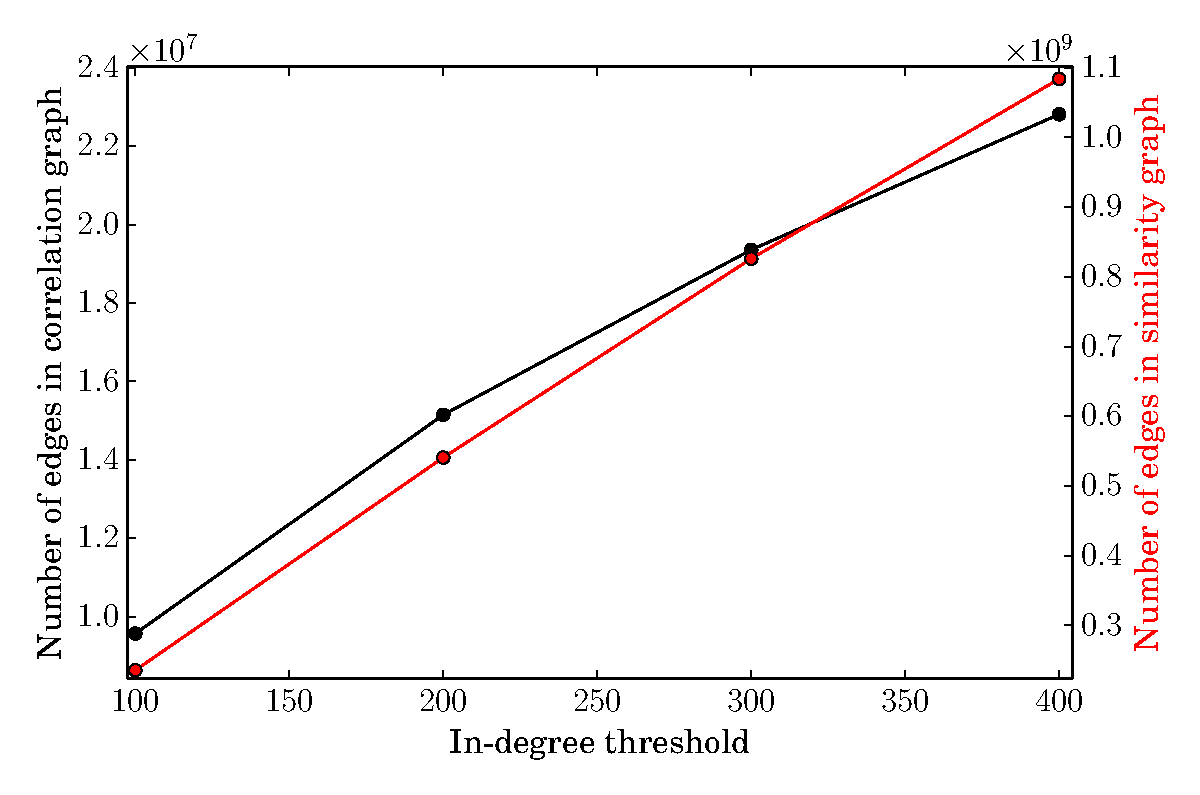
\includegraphics[width=0.75\columnwidth]{figures/eng-all-edge-low-e3-vtx-low-e8-high-e1-100-400-idg-ne-nt.pdf}}
\caption{Number of edges in the correlation- and similarity graph, respectively, for different in-degree thresholds. Built from Google Books 5-grams
with the same configuration as in Fig.\ \ref{fig:google-e-runtime}.}
\label{fig:google-ne}
\end{figure}

\begin{table}
\renewcommand{\arraystretch}{1.3}
\caption{Runtimes in seconds for Google Books dataset.}
\label{tab:google_runtimes}
\begin{center}
\begin{tabular}{c|r|r|r||c|c}
  \hline \bfseries In-degree  & \bfseries Run 1
  & \bfseries Run 2
  & \bfseries Run 3
  & \bfseries $\mu$
  & \bfseries $\sigma$
  \\
  \hline\hline 100
  & 246.7
  & 229.5
  & 236.7
  & 237.6
  & 8.6
  \\
  \hline 200
  & 603.7
  & 573.2
  & 575.4
  & 584.1
  & 16.9
  \\
  \hline 300
  & 1062.4
  & 998.3
  & 1031.2
  & 1030.7
  & 32.0
  \\
  \hline 400
  & 1535.5
  & 1602.5
  & 1554.0
  & 1564.0
  & 34.6
  \\
  \hline
\end{tabular}
\end{center}
\end{table}

\section{Conclusions}
\label{sec:conclusions}

This paper proposes conceptually simple methods for discovering similarities and concepts by 
transforming a correlation graph to a similarity graph on which clustering is performed. As the approach does not rely on any
intermediate representation or dimensionality reduction, or on specific information about objects besides
their correlations, it is applicable with few restrictions
to any domain in which a correlation graph can be constructed. Our experiments show that the approach not only can
detect similarities and concepts in several types of data, but also that it is computationally feasible for large-scale
applications with very large numbers of objects and correlations.

Due to the generality of the approach there is a vast number of possible directions to take. For instance, it can 
potentially be used to discover analogous objects in gene regulatory data or protein interaction networks, to provide 
recommendations from user data, or in general for detecting higher-order dynamics in 
discrete-valued stochastic processes. It then remains to quantitatively evaluate the properties of the scheme, for example in 
terms of application specific benchmark performance, approximation error and runtime. 

The main methodological challenge for future work revolves around how to efficiently build hierarchical concept models.
The concepts discovered through the methods described in this paper essentially represent OR-relations: All constituent
objects of a cluster are commutable, and the concept can be said to be observed if any of its constituents
are. Analogously, strong clusters detected in the correlation graph could be considered to represent AND-relations,
where the corresponding concept is observed when all of its constituents are. Both these types of
concepts can be identified, brought back into the estimation of the correlation graph, and the process
iterated, allowing for the discovery of complex higher-order relations. How to reliably and efficiently perform this
remains an area of further study.

\begin{acknowledgements}
This work was funded by the Swedish Foundation for Strategic Research (\emph{Stiftelsen f\"or strategisk forskning}) 
and the Knowledge Foundation (\emph{Stiftelsen f\"or kunskaps- och kompetensutveckling}). 
The authors would like to thank the anonymous reviewers for their valuable comments.\end{acknowledgements}

\bibliography{concepts-kais}

%\section*{Author Biographies}
%\leavevmode

%\vbox{%
%\begin{wrapfigure}{l}{80pt}
%{\vspace*{15pt}\fbox{insert photo}\vspace*{100pt}}%
%\end{wrapfigure}
%\noindent\small 
%{\bf Li Shen} received a B.E. degree from Xi'an Jiao Tong University,
%Xi'an, China, in 1993 and an M.E. degree from Shanghai Jiao Tong
%University, Shanghai, China, in 1996.  >From 1997 to 1998, he did
%research work in the Data Mining Group at the School of Computing and
%Information Technology, Griffith University, Brisbane, Australia.  He
%is currently a Ph.D. student at the Department of Computer Science,
%Dartmouth College, USA. His research interests include data mining,
%multimedia, database and software engineering.\vadjust{\vspace{40pt}}}
%
%\vbox{%
%\begin{wrapfigure}{l}{80pt}
%{\vspace*{15pt}\fbox{insert photo}\vspace*{100pt}}%
%\end{wrapfigure}
%\noindent\small {\bf Hong Shen} is currently Associate Professor
%(Reader) in the School of Computing and Information Technology and
%Research Director of Parallel Computing Unit at Griffith
%University. He held visiting posts in several leading universities in
%USA, Europe and Asia. With main research interests in algorithms,
%parallel and distributed computing, interconnection networks, parallel
%databases and data mining, multimedia systems and networking, he has
%authored over 120 technical papers.  Dr Shen has served as an editor
%of the {\it Journal of Parallel and Distributed Computing Practice},
%associate editor of the {\it International Journal of Parallel and
%Distributed Systems and Networks}, and on the editorial board of the
%{\it Journal of Parallel Algorithms and Applications}, {\it
%International Journal of Computer Mathematics} and the {\it Journal of
%Supercomputing}. He has been involved in organization of various
%international conferences.}
%
%\vspace{15pt}
%\vbox{%
%\begin{wrapfigure}{l}{80pt}
%{\vspace*{15pt}\fbox{insert photo}\vspace*{100pt}}%
%\end{wrapfigure}
%\noindent\small 
%{\bf Ling Cheng} received a B.E. degree from Xi'an Jiao Tong
%University, Xi'an, China, in 1993 and an M.E. degree from Shanghai
%Jiao Tong University, Shanghai, China, in 1996. From 1996 to 1997, she
%worked in the IBM China Research Lab, Beijing, China.  In 1998, she
%was a visiting scholar at the School of Computing and Information
%Technology, Griffith University, Brisbane, Australia.  She is
%currently a graduate student at the Department of Computer Science,
%Dartmouth College, USA. Her research interests include data mining,
%multimedia, database and e-commerce.}
%
%\vspace{15pt}
%\vbox{%
%\begin{wrapfigure}{l}{80pt}
%{\vspace*{15pt}\fbox{insert photo}\vspace*{100pt}}%
%\end{wrapfigure}
%\noindent\small 
%{\bf Paul Pritchard} is currently Professor in the School of Computing
%and Information Technology and Executive Director of the Parallel
%Computing Unit at Griffith University. He is also joint Manager of
%Queensland Parallel Supercomputing Facility (QPSF) and served as Head
%of the school (1991--1993), and Dean of Faculty of Information and
%Communication Technology (1997--1999).  With main research interest in
%algorithms, programming languages, high-performance computing,
%Internet computing and data mining, Professor Pritchard has published
%numerous papers in several areas of computer science. He is best known
%for his contributions to number-theoretic algorithms, and his wheel
%sieve is the fastest known algorithm for enumerating the prime
%numbers.  He is foundation editor of the {\it Journal of Universal
%Computer Science}, and has chaired several conferences.}

\correspond{Olof G\"{o}rnerup, Swedish Institute of Computer Science (SICS),
SE-164 29 Kista, Sweden. Email: olof@sics.se.}
\label{lastpage}
\end{document}
